\documentclass[UTF8,12pt,a4paper]{ctexart}
\usepackage[a4paper,margin=2.25cm,headheight=15pt]{geometry}
\usepackage{amsmath,amssymb,bm}
\usepackage{booktabs,array,tabularx,longtable}
\usepackage{graphicx,float,caption}
\usepackage{xcolor,tikz,hyperref,siunitx}
\usetikzlibrary{arrows.meta,positioning,calc}
\definecolor{navy}{HTML}{153A5B}
\definecolor{blue}{HTML}{2E75B6}
\definecolor{green}{HTML}{2E7D5B}
\definecolor{orange}{HTML}{C76A20}
\hypersetup{colorlinks=true,linkcolor=navy,urlcolor=blue}
\setlength{\parindent}{2em}
\setlength{\parskip}{0.28em}
\setlength{\emergencystretch}{2em}
\captionsetup{font=small,labelfont=bf}
\sisetup{detect-all}

\begin{document}
\begin{titlepage}
\centering
\vspace*{2.0cm}
{\Huge\bfseries\color{navy} 分段策略对高频变压器\\宽频响应与内部电压保持能力的影响\par}
\vspace{0.8cm}
{\Large EXP-012 详细实验报告\par}
\vspace{1.5cm}
\begin{tikzpicture}[node distance=0.55cm,>=Latex,scale=0.72,transform shape]
\node[draw=blue,rounded corners,fill=blue!8,minimum width=3.2cm,minimum height=1cm] (fine) {24+24 细单元参照模型};
\node[draw=orange,rounded corners,fill=orange!8,right=of fine,minimum width=3.0cm,minimum height=1cm] (seg) {三种连续分段策略};
\node[draw=green,rounded corners,fill=green!8,right=of seg,minimum width=3.0cm,minimum height=1cm] (reduce) {结构保持能量聚合};
\node[draw=navy,rounded corners,fill=navy!7,right=of reduce,minimum width=3.0cm,minimum height=1cm] (eval) {端口/模态/内部应力评价};
\draw[->,thick] (fine)--(seg); \draw[->,thick] (seg)--(reduce); \draw[->,thick] (reduce)--(eval);
\end{tikzpicture}
\vfill
\begin{tabular}{rl}
\textbf{实验分支：}& \texttt{work/experiments}\\
\textbf{频率范围：}& \SI{1}{kHz}--\SI{10}{MHz}，321 个对数频点\\
\textbf{分段规模：}& 每绕组 $2,4,6,8,12$ 段\\
\textbf{报告日期：}& 2026年8月17日
\end{tabular}
\vfill
{\large 本报告描述合成无源模型上的方法验证，不代表特定样机的物理精度。\par}
\end{titlepage}

\begin{abstract}
本实验针对高频变压器分段梯形网络中“如何选择分段位置”这一问题，建立原、副边各24个细单元的常参数无源参照模型，并将其压缩为每绕组2、4、6、8和12段的粗模型。比较策略包括均匀分段、按非均匀绕组层边界分段，以及由内部电压响应和局部绕组间电容端口灵敏度共同引导的连续分段。所有粗模型采用同一结构保持聚合规则，不重新拟合参数。结果显示，端口导纳误差对分段位置不敏感，可低至$10^{-5}\%$量级；但内部相邻电压应力误差在低阶模型中可超过$10\%$。因此，仅凭端口拟合精度无法证明内部状态保真。在本次事后设定的试探性精度阈值下，信息引导模型从每绕组8段开始同时满足端口、关键模态、内部峰值和相邻电压应力要求。该结论支持继续开展“端口Fisher信息引导的连续分段”，但尚需独立参数集、FEM和样机验证。
\end{abstract}

\tableofcontents
\newpage

\section{实验目的与研究问题}
现有集中参数模型可辨识总漏感和总绕组间电容，但无法描述局部电压应力和局部参数变化。直接增加梯形单元又会造成参数数量膨胀和端口不可辨识。本实验首先回答：在固定逐匝参照模型的条件下，分段数与分段位置如何共同影响外部端口响应、关键内部模态和电压应力保持能力？

本实验不进行DAB参数反演。它为下一阶段提供经过筛选的粗模型结构，避免把模型降阶误差和反演误差混在一起。

\section{逐匝参照模型}
设每个绕组包含$n=24$个细单元，支路电流向量为$\bm i_b\in\mathbb C^{2n}$，节点电压为$\bm v\in\mathbb C^{2n}$。参照模型由
\[
\bm Z_b(\omega)=\bm R+j\omega\bm L
\]
和Maxwell型节点电容矩阵$\bm C$构成。支路--节点关联矩阵记为$\bm A$，完整节点导纳为
\begin{equation}
\bm Y_f(\omega)=\bm A\bm Z_b^{-1}(\omega)\bm A^T+j\omega\bm C.
\end{equation}
模型保留全电感耦合、纵向电容、对地电容以及高斯空间核形式的完整原副边电容耦合。为保证无源性，构造时强制满足
\[
\bm R\succ0,\qquad \bm L=\bm L^T\succ0,\qquad \bm C=\bm C^T\succ0.
\]
数值检查得到$\lambda_{\min}(\bm L)=7.199\times10^{-9}\,\mathrm H$，$\lambda_{\min}(\bm C)=6.093\times10^{-13}\,\mathrm F$，两矩阵对称残差均为0。

\section{结构保持粗化推导}
\subsection{连续分段与映射矩阵}
给定连续边界
\[
0=b_0<b_1<\cdots<b_m=n,
\]
同一粗单元内的细支路串联，因而共享粗支路电流。定义支路电流嵌入矩阵$\bm T$，使
\[
\bm i_f\approx\bm T\bm i_c.
\]
节点电压使用分段线性延拓矩阵$\bm P$：
\[
\bm v_f\approx\bm P\bm v_c.
\]
最终参考节点保持为零电位，外部两个端口节点保持不变。

\subsection{能量等效参数聚合}
由电阻损耗、磁场能量和电场能量守恒，粗模型参数统一写成
\begin{align}
\bm R_c&=\bm T^T\bm R\bm T,\\
\bm L_c&=\bm T^T\bm L\bm T,\\
\bm C_c&=\bm P^T\bm C\bm P.
\end{align}
粗模型节点导纳为
\begin{equation}
\bm Y_c(\omega)=\bm A_c(\bm R_c+j\omega\bm L_c)^{-1}\bm A_c^T+j\omega\bm C_c.
\end{equation}
该模型可脱离逐匝模型独立求解；逐匝模型只在离线阶段用于构造$\bm R_c,\bm L_c,\bm C_c$。

\subsection{端口消元与内部电压恢复}
将节点分为端口$p$和内部节点$i$：
\[
\begin{bmatrix}\bm i_p\\0\end{bmatrix}=
\begin{bmatrix}\bm Y_{pp}&\bm Y_{pi}\\\bm Y_{ip}&\bm Y_{ii}\end{bmatrix}
\begin{bmatrix}\bm v_p\\\bm v_i\end{bmatrix}.
\]
因此
\begin{align}
\bm Y_{\mathrm{port}}&=\bm Y_{pp}-\bm Y_{pi}\bm Y_{ii}^{-1}\bm Y_{ip},\\
\bm v_i&=-\bm Y_{ii}^{-1}\bm Y_{ip}\bm v_p,\\
\hat{\bm v}_f&=\bm P\bm v_c.
\end{align}

\section{三种分段策略}
\subsection{均匀分段}
按几何序号等长划分，作为最简单基线。

\subsection{物理层分段}
预设非均匀层尺寸$[4,7,5,8]$，优先保留层边界；当粗单元数超过层数时，再按层长度分配额外单元。

\subsection{信息引导连续分段}
每个细位置构造特征
\[
\bm\phi_i=[\text{双端口激励下内部复电压响应},\ \partial\bm Y_{\rm port}/\partial\log C_{ps,i}],
\]
对特征进行尺度归一化后，计算相邻位置跳变量
\[
d_i=\frac{\|\bm\phi_{i+1}-\bm\phi_i\|_2}{\sqrt{N_\phi}}.
\]
优先在$d_i$较大的位置设置分段边界，并使用间距惩罚避免多个边界聚集。该版本强制只能合并相邻匝，保持梯形拓扑。

需要强调：当前特征包含细模型内部电压，属于离线oracle信息。后续应拆分为oracle上限和仅使用端口Fisher信息的可部署版本。

\section{评价指标}
端口相对误差采用全频带Frobenius范数：
\[
E_Y=\frac{\|\bm Y_{c,\mathrm{port}}-\bm Y_{f,\mathrm{port}}\|_F}{\|\bm Y_{f,\mathrm{port}}\|_F}.
\]
关键模态由无损广义特征值问题获得：
\[
\bm A\bm L^{-1}\bm A^T\bm q_r=\omega_r^2\bm C\bm q_r,
\]
并按端口参与因子选择频带内最重要的六个模态。内部指标包括排除固定外部端口后的全局峰值误差、峰值位置，以及相邻细支路最大电压差误差。

本次试探阈值为：$E_Y\le0.2\%$、关键模态误差$\le0.01\%$、内部峰值误差$\le0.1\%$、相邻电压应力误差$\le1\%$。这些阈值是在初步运行后设定，只用于本轮方法筛选，不是预注册确认性判据。

\section{实验结果}
\begin{figure}[H]
\centering
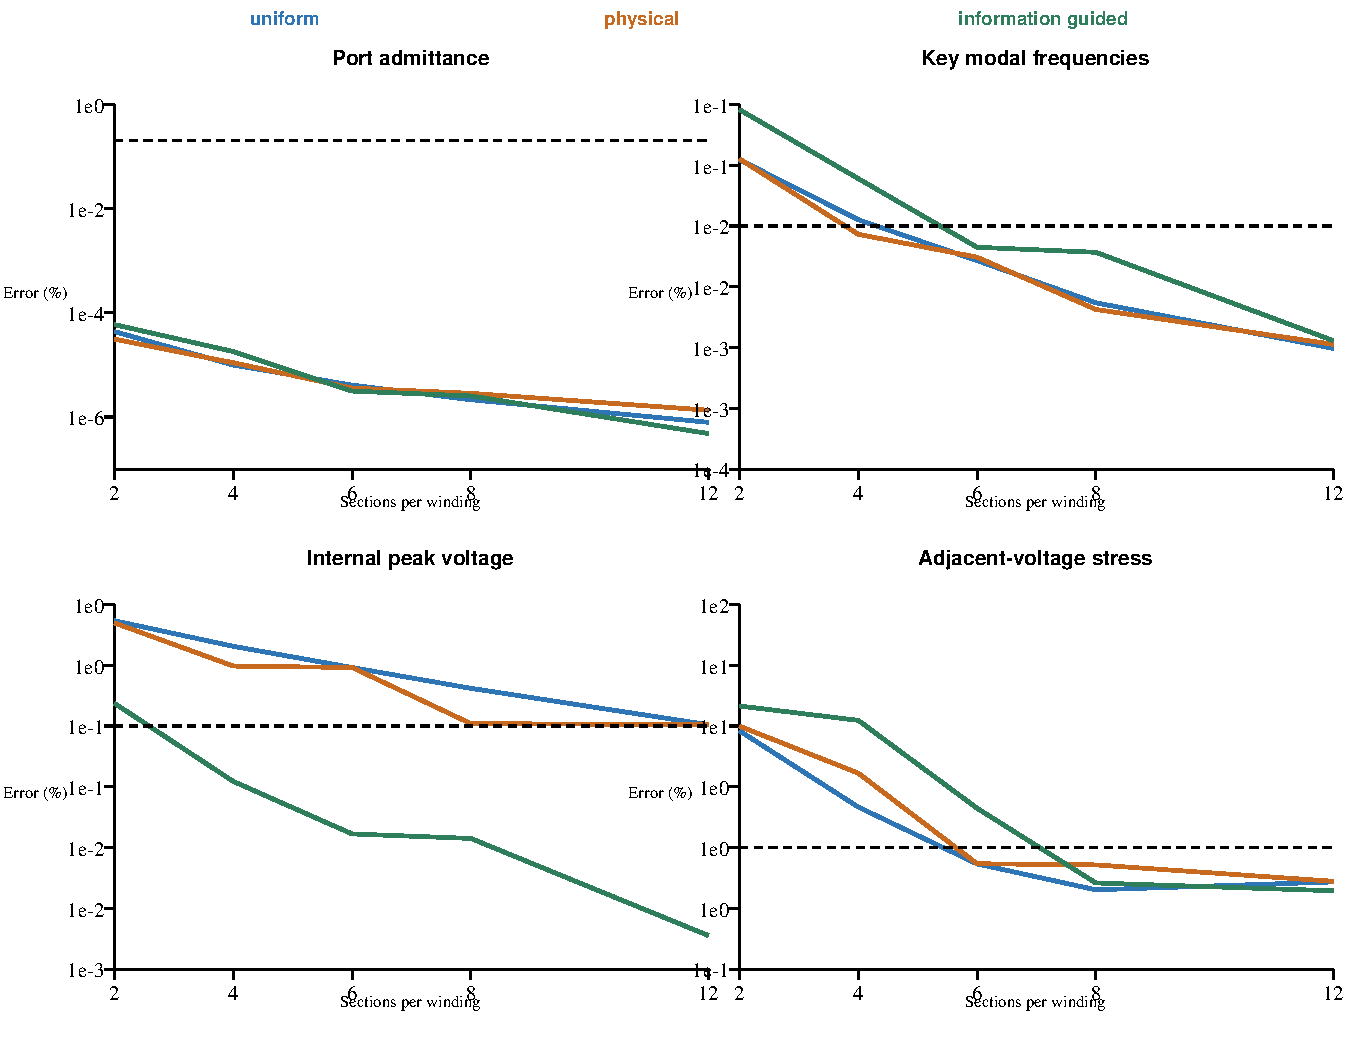
\includegraphics[width=\textwidth]{figures/segmentation_comparison.pdf}
\caption{三种连续分段策略随粗单元数变化的误差。纵轴使用对数尺度，黑色虚线为本轮试探阈值。}
\end{figure}

\begin{table}[H]
\centering
\caption{代表性分段结果（误差单位：\%）}
\small
\begin{tabular}{llrrrrr}
\toprule
策略 & 每绕组段数 & 端口 & 模态 & 内部峰值 & 相邻应力 & 加速比\\
\midrule
均匀 & 2  & $4.36\!\times\!10^{-5}$ & 0.0351 & 0.7346 & 9.121 & 4.59\\
物理 & 4  & $1.10\!\times\!10^{-5}$ & 0.0085 & 0.3113 & 4.092 & 4.43\\
信息引导 & 6 & $3.15\!\times\!10^{-6}$ & 0.0067 & 0.0129 & 2.106 & 4.11\\
信息引导 & 8 & $2.54\!\times\!10^{-6}$ & 0.0061 & 0.0119 & 0.511 & 3.58\\
均匀 & 12 & $7.91\!\times\!10^{-7}$ & 0.0010 & 0.1025 & 0.521 & 3.08\\
信息引导 & 12 & $4.81\!\times\!10^{-7}$ & 0.0011 & 0.0019 & 0.441 & 3.07\\
\bottomrule
\end{tabular}
\end{table}

每绕组8段的信息引导边界为
\[
[0,1,5,6,9,11,18,21,24],
\]
它保留了首端快速变化位置以及若干内部特征突变位置，是测试集合中最小的全指标达标模型。均匀和物理策略即使达到12段，内部峰值误差仍略高于本轮$0.1\%$阈值。

\section{结果解释}
\subsection{端口正确不等于内部正确}
所有策略的端口误差均非常小，但2段模型的相邻电压应力误差达到$9\%$--$15\%$。因此，如果只用$Y_{11},Y_{12},Y_{22}$拟合误差评价分段模型，会高估粗模型对内部绝缘应力的描述能力。这一结果为后续同时使用端口Fisher信息和内部风险代理指标提供了依据。

\subsection{信息引导并非在所有低阶规模上都最好}
信息引导2段和4段模型为了保留首端内部电压特征，将大量剩余细单元合并，反而放大另一端的相邻电压应力误差。因此合理结论不是“信息引导必然优于均匀分段”，而是信息引导必须与最小单元宽度、应力误差或多目标动态规划结合。

\subsection{计算时间解释}
逐匝48维模型的321频点求解在重复运行中约为\SI{0.06}{s}--\SI{0.10}{s}；粗模型约\SI{0.01}{s}--\SI{0.03}{s}，代表性加速比约为3--7倍。表中列出报告生成轮次的计时值。该计时会受缓存和系统负载影响，仅反映当前小规模NumPy线性代数实现，不应外推到大型FEM或开关级DAB仿真。

\section{本实验已经证明与尚未证明的内容}
\subsection*{已经证明}
\begin{enumerate}
\item 可以从同一无源逐匝矩阵构造独立、无源的粗梯形网络；
\item 分段位置会显著影响内部峰值和相邻电压应力保持能力；
\item 极小的端口误差不能保证内部状态准确；
\item 在当前合成模型和试探阈值下，信息引导8段模型是最小全指标达标模型。
\end{enumerate}

\subsection*{尚未证明}
\begin{enumerate}
\item 尚未证明该分段策略适用于真实高频变压器；
\item 尚未使用FEM或实测参数标定$\bm R,\bm L,\bm C$；
\item 尚未在DAB多运行窗口下反演局部参数；
\item 尚未证明仅靠外部端口Fisher信息可以复现当前oracle边界；
\item 尚未进行独立随机种子、参数族和跨样机泛化验证。
\end{enumerate}

\section{下一步实验建议}
下一版不应立即加入深度学习。建议先完成EXP-012B：固定相同逐匝模型族，分别构造oracle内部模态分段、仅端口Fisher分段和多目标动态规划分段；使用独立参数集评价分段边界。随后进入EXP-013，在选定的8段模型上仅辨识
\[
\bm\theta=[L_{\sigma,1},L_{\sigma,2},C_{ps,1},C_{ps,2}]^T,
\]
检查Fisher秩、最小特征值、条件数和灵敏度列相关性，并与全局$L_s,C_{ps}$模型比较。

\appendix
\section{可复现文件}
\begin{itemize}
\item \texttt{config.json}：固定随机种子、频率网格和分段规模；
\item \texttt{segmentation\_experiment.py}：模型、分段、粗化、求解和指标；
\item \texttt{results/segmentation\_metrics.csv}：15组完整指标；
\item \texttt{results/experiment\_summary.json}：汇总结论；
\item \texttt{results/reference\_model\_matrices.npz}：参照矩阵原始数据；
\item \texttt{make\_figures.py}：矢量图生成脚本。
\end{itemize}

\end{document}
